\section{Towards a Database Evolution Framework}
	\label{sec:def}

% Introduce development lifecycle and show that happens multiple time

Our framework approach is based on some key concepts and some hypothesis. First of them is that the solution developed and managed lied on 

As we have read, usually, Database administrator do not like to change any database schema due to the risk implied by the changes. One minor change at a point of schema could have major repercussions to the whole system you have. In our case, we have only one application per database. This is the ideal case that any DBA dream about it. When you change your code, you can change your database relatively easily due to the fact there is only this application that use the database. You do not impact any other application. You could have one or two exception when you have some reporting application that directly interrogate your database.

With our approach, we want to cover a relative basic approach. We suppose that only one application is concerned by a migration process with no exception (other external data extracting tools). On this base, we are able to build a framework with different identified people, process rules and tools that all together bring a way to handle as best as possible the migration whole process. We also based our processes and tools on the fact that the application use an ORM\cite{orm} that brings high development capabilities but a loss in control in your database access. With the persistence layer that the ORM brings, you have not necessarily the control of the underlying relational data model but you, normally, do not have to write any SQL\cite{sql} in your application. We do this hypothesis that we do not use any native SQL language inside the application. With these differents hypothesis, we do not realize that any change in our data model will greatly implies an impact on our database schema or data.

Let's start with a discussion about the people involved in the process of data migration. We are interested by identifying the role of people in such a way to know what they do in the process and/or what their impacts on the data evolution. We will discuss also about when they step in the lifecycle. When we have an overview of these roles, we could introduce the processes used and who manage them. Finally, to help in the application of the process, we need tools. Some of them are written to suit the processes we offer.

\subsection{People}
	\label{sec:def:people}

We have identified different kind of people that are implied in the whole process of the data migration.

\subsubsection{Customer\\}

The most important people are the customers. Without them, we do not have any business. This is an evidence. They ask for new features, they ask for improvements, they ask for corrections. They are at the center of any evolution triggered by the market needs. When they ask such of modifications, they have no idea of the technical impacts and they do not want especially to be involved with this kind of things. They just want that our product reach their requirements.

\subsubsection{Product owner\\}

The product owner is in charge to manage the evolution of the product. He has a good knowledge of the market and try to anticipate the market needs. He wants that the product evolves to get new customers but also to satisfy current customers. He tries to balance the current features with the new features to introduce to match new requirements from old and new customers. In this position, he has a great interaction with developers due to the fact he basically gives the tasks to developers.

\subsubsection{Project manager\\}

When you offered an application as a service, you have sometimes to integrate partners. These integrations are, in general, managed as projects. We could see this organization as a transverse one. In facts, the project has an impact on the application. The project manager has the same kind of power than a product manager. He tries to balance the requirements of customers and partners to conserve the coherence of the application. He also gives tasks to developers that imply sometimes database evolution. He has a great implication with the product owner.

\subsubsection{Developer\\}
	\label{sec:def:developer}

A developer is the person that have the most impact in terms of technical aspects. He introduces the changes inside the application source code that have the impact on the database. For this reason, this is also the person that is the best placed to know exactly which kind of modification he did and how to handle it. For these reasons, the developer has an important task when he did a modification that impact the database. He has to write migration scripts relating to his modification. He must test them to ensure that the scripts are runnable.

\subsubsection{Migration manager\\}

The migration manager has the role of coordination to follow the migration scripts writing. He tries to know all about the application, to know any change in the data model of the application. He does a first migration scripts review in terms of concern separation. He needs to separate contextual modifications from technical ones. He keeps the scripts organization as cleaner as possible. Finally, he tries to catch missing scripts or erroneous ones. His role is more in coordination than technical. He could also have the role of developer in writing scripts. He must be an example by following the rules and teaches them to others.

\subsubsection{Database administrator\\}

Database administrators manage the databases for performances, integrity, maintenance operations. But he has also an important role of migration code review. He must be able to get the migrations scripts written by developers to run them. He must be able to validate that the scripts technically run against a database that must be upgraded. He is also there to give feedbacks to developers when the migration scripts must be improved due to lack of performances. 

\subsubsection{System administrator\\}

The system administrator, in addition of maintaining the system running, has in charge the application migration. With the help of DB Administrators, he has to run the migration scripts during the application migration. He must provide sandbox environments for migration testing in the most nearest production way as possible. The application migration must be run in the nearest real conditions. He ensures the execution of the migration process. He will also do the migration on the real environments when the sandbox ones will be validated by Quality Assurance team.

\subsubsection{Quality assurance agent\\}

To ensure the migration keep the application correct and functional from end user point of view, we need people able to run manual and automatic tests agains the migrated application. The quality assurance agent has the responsibility to test the application after a migration and validates that technical all is correct but also from business point of view. He needs to validate that the application reacts as the customers asked and also ensure that all data keep integrity, no data loss, no side effects on the data. He will give the ok/nok for the production application migration. The quality assurance agent could be internal people or external people. Customers could provide their quality assurance agents to keep a regard on the migration process.

\subsubsection{End user\\}

The end user is the person that use the application offered by our customers. We do not address directly the end user but we have a big incidence for their user experience. With their feedbacks to our customers, we will have corrections and/or improvements. At all, the migration process starts and ends with the end users inputs (directs or indirects). Any process has its weakness. 

\subsubsection{Summary}

We can summarize the previous roles as stories to help us in the definition of the process part.

\begin{itemize}
\renewcommand{\labelitemi}{$\bullet$}
\item As a customer, I want to be sure that a new version of the system do not corrupt actual data
\item As a customer, I want to be sure new features are implemented as I need and will use data correctly
\item As a product owner, I want the insurance that the system keep the correctness of data after migration
\item As a product owner, I want to be sure that the requirements based on the data already present in the application
\item As a project manager, I have the same concerns as a product owner
\item As a project manager, I want to have the insurance that our data are equivalent to partners data when we need reconciliation
\item As a developer, I want to develop with ease and flexibility without worrying to much about the data migration.
\item As a developer, I need a way to write migration scripts quite easily with well defined procedures
\item As a migration manager, I want to keep a trace of the data model modification or any database relating updates
\item As a migration manager, I need tools to help me to track changes and to build final migration scripts
\item As a migration manager, I need to have procedure to follow migration scripts writing progress
\item As a database administrator, I want to be sure that I can dispose migration scripts when it is necessary
\item As a database administrator, I need to run the migration scripts at any time to do testing and ask for improvements
\item As a system administrator, I want to be sure that the application migration could be done with the minimal risk of migration rollback
\item As a system administrator, I will provide sandbox environments to test migration scripts and application migration
\item As a system administrator, I run the application migration on the different environments (with/without help of DB Admistrator)
\item As a QA agent, I want to have the possibility to test the application after migration in a sandbox environment
\item As a QA agent, I need to automatize the tests to have a more complete testing process
\item As a QA agent, I will give the go or no go to a production application migration (with the approval of customers)
\item As an end user, I want to have the best user experience without worrying about the technologies used to offer me the services I used
\item As an end user, I do not want to encounter major issues due to application updates
\end{itemize}

\subsection{Process}
	\label{sec:def:process}

Our framework relies on processes and tools that we combine to manage the different database evolution. For the next paragraphs, we assume that a code versioning system is used to manage the code. This system is able to use a plugin system to add some actions at different point in the versioning process such code is manipulated in the versioning system. The framework is agnostic for the choice of such a system or which database engine used by the application.

The process to manage the migration process requires several steps. First of all, it is necessary to monitor the code modification to detect any change that could imply a database evolution. After that, we need to ensure that the migration scripts are written and correct. Then, we need to run the migration script on a sandbox environment to ensure the correctness on a database that contains data in production way. Finally, when all is fine, we could run the migration on the production environment. The Fig. \ref{fig:migrationProcess} summarize the migration process.

\begin{figure}[h]
        \centering
        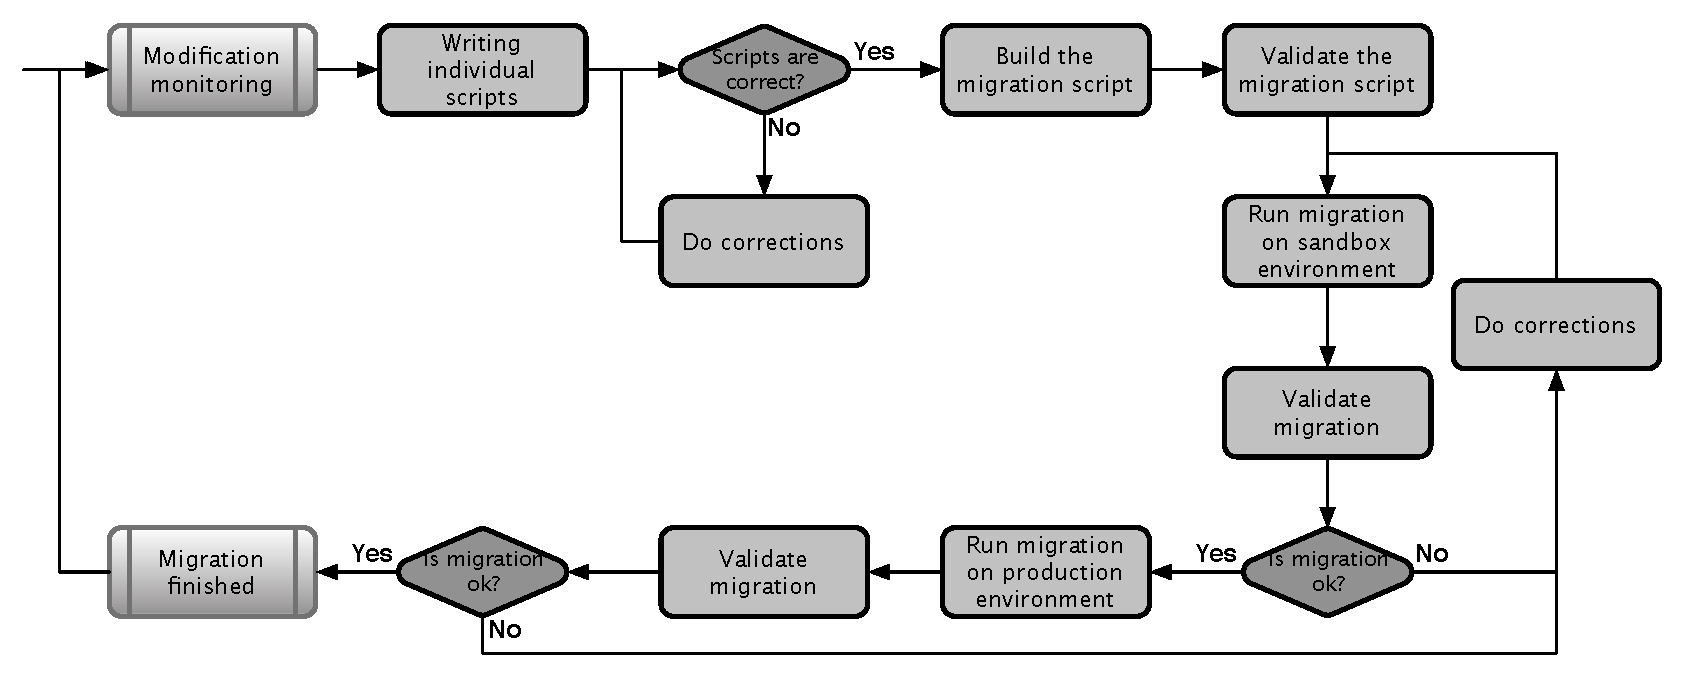
\includegraphics[scale=0.50]{images/MigrationProcess.pdf}
        \caption{Migration process}
        \label{fig:migrationProcess}
\end{figure}

One part of the whole process of data migration is to track the data model transformations. As we know, we have defined different kind of data transformation. We have structural refactoring that implies schema transformation (adding a column, adding a table, removing column, data type modification and so on). We have data migration that imply to work on the data present in the database. In this case, we can divide in two groups, the data that are generic (called infrastructural data) and data that are used in the application deployment (called contextual data). Depending on which transformations, the migration process is slightly different and more work is required to ensure correct evolution. For further details, refer to \autoref{sec:risks}.

When the modification are tracked, it is important to check the migration writing process and to enforce some rule for the migration scripts writing. On the Fig. \ref{fig:migDetProc}, we suggest a process to monitor and ensure that the migration scripts are written and are correct. Basically, the first step for this process is the monitoring of the data model modifications. When such a modification is caught, a short analysis is done to ensure if a script is required for the modification detected or not. If a modification is required, another process is required to ensure that the migration is correct and follows the migration writing rules. Finally, all this monitoring is kept in a file to track at any time the state of the migration scripts. We offer a format that could be used for that in Fig. \ref{fig:migTemplate}.

At this point, the migration monitoring process will be done regularly to avoid any delays in the migration writing process to ensure that at any time, the migration scripts to deploy the applications could be built from the migrations script parts.

\subsubsection{Tracking model modification\\}

As we just discussed previously, one important part of our approach is the data model monitoring to track any modification. This part use actively on the versioning tool in place. In general, these kind of tools allows to add sort of plugins to do extra work after or before any piece of code is injected into the versioning repository. These functionnalities offers a great way to automate some controls. Some scripts can verify if any piece of code could be eligible for a migration scripts. With basic checks, emails could be sent to a mailing list for a further analysis. Some updates could simply comments in the code that are not a modification that requires a migration script.

\begin{figure}[h]
        \centering
        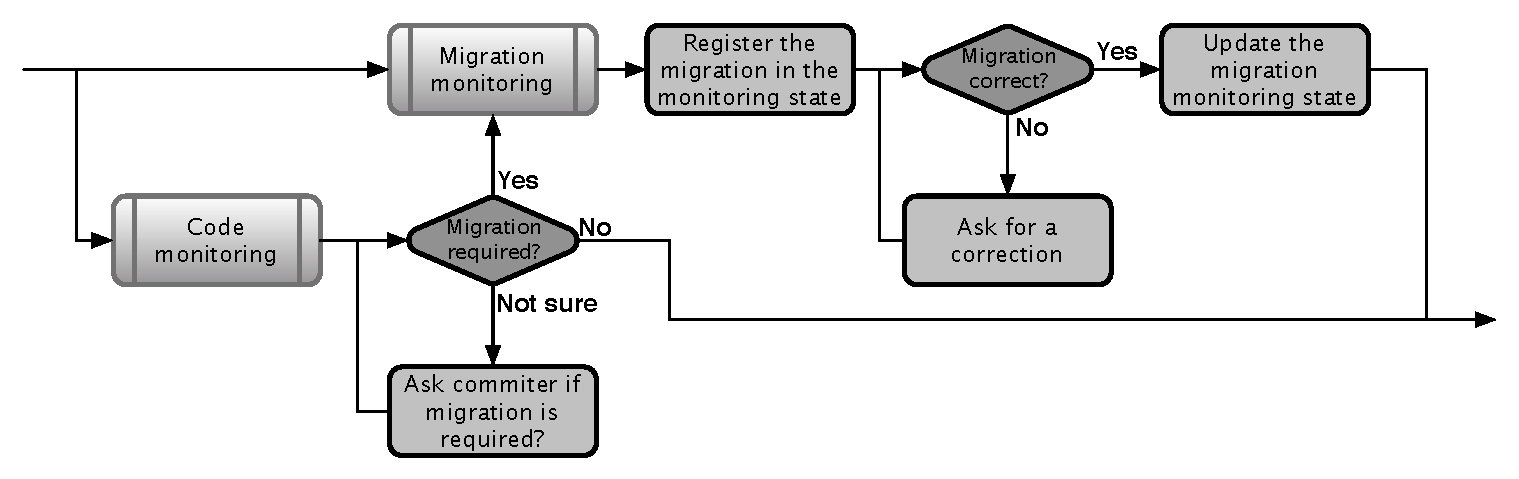
\includegraphics[scale=0.55]{images/MigrationDetetcionProcess.pdf}
        \caption{Migration monitoring process}
        \label{fig:migDetProc}
\end{figure}

When a modification is eligible for a migration script, the migration tracking file must be updated for the revision that contains the modification. The first two columns could be filled with the migration number (basically an incremental number) in the current migration process and the migration name. The commiter column must be filled too.

At this stage, the migration monitoring could start. Each developer that produces a modification that requires a migration needs to write the corresponding migration script. For that, the developers relays to the migration script writing rules described a little bit later in this paper. In the same way that the code modification are monitored, we could do the same for the migration scripts. The first reason is to know that the migration script file is created, when it is created and by which. The second reason allows checking the migration script regularly. This is important to check the correctness of the scripts and ask quickly for modifications if required. A third reason is to check that a script is not modified frequently and for the bad reasons. A migration script must be immutable. It means that we do not want any modifications of scripts expect for corrections. For this step, the columns "Present" and "Correct" are used to know the state of the migration script. The "Remarks" column is a quick help to keep the reason why a script is correct for example. The "Added in" column is filled with the revision identifier when the migration script was commited to the versioning repository.

We also use a "Releated to" column to track the contextual migration in regards of the modifications done in the code. We want to keep the context of the migration and for that we need to know for which revision identifiers the migration is relevant. We will discuss in depth this last part and the naming rules in the section \autoref{sec:rules}.

\begin{figure}[h]
        \centering
        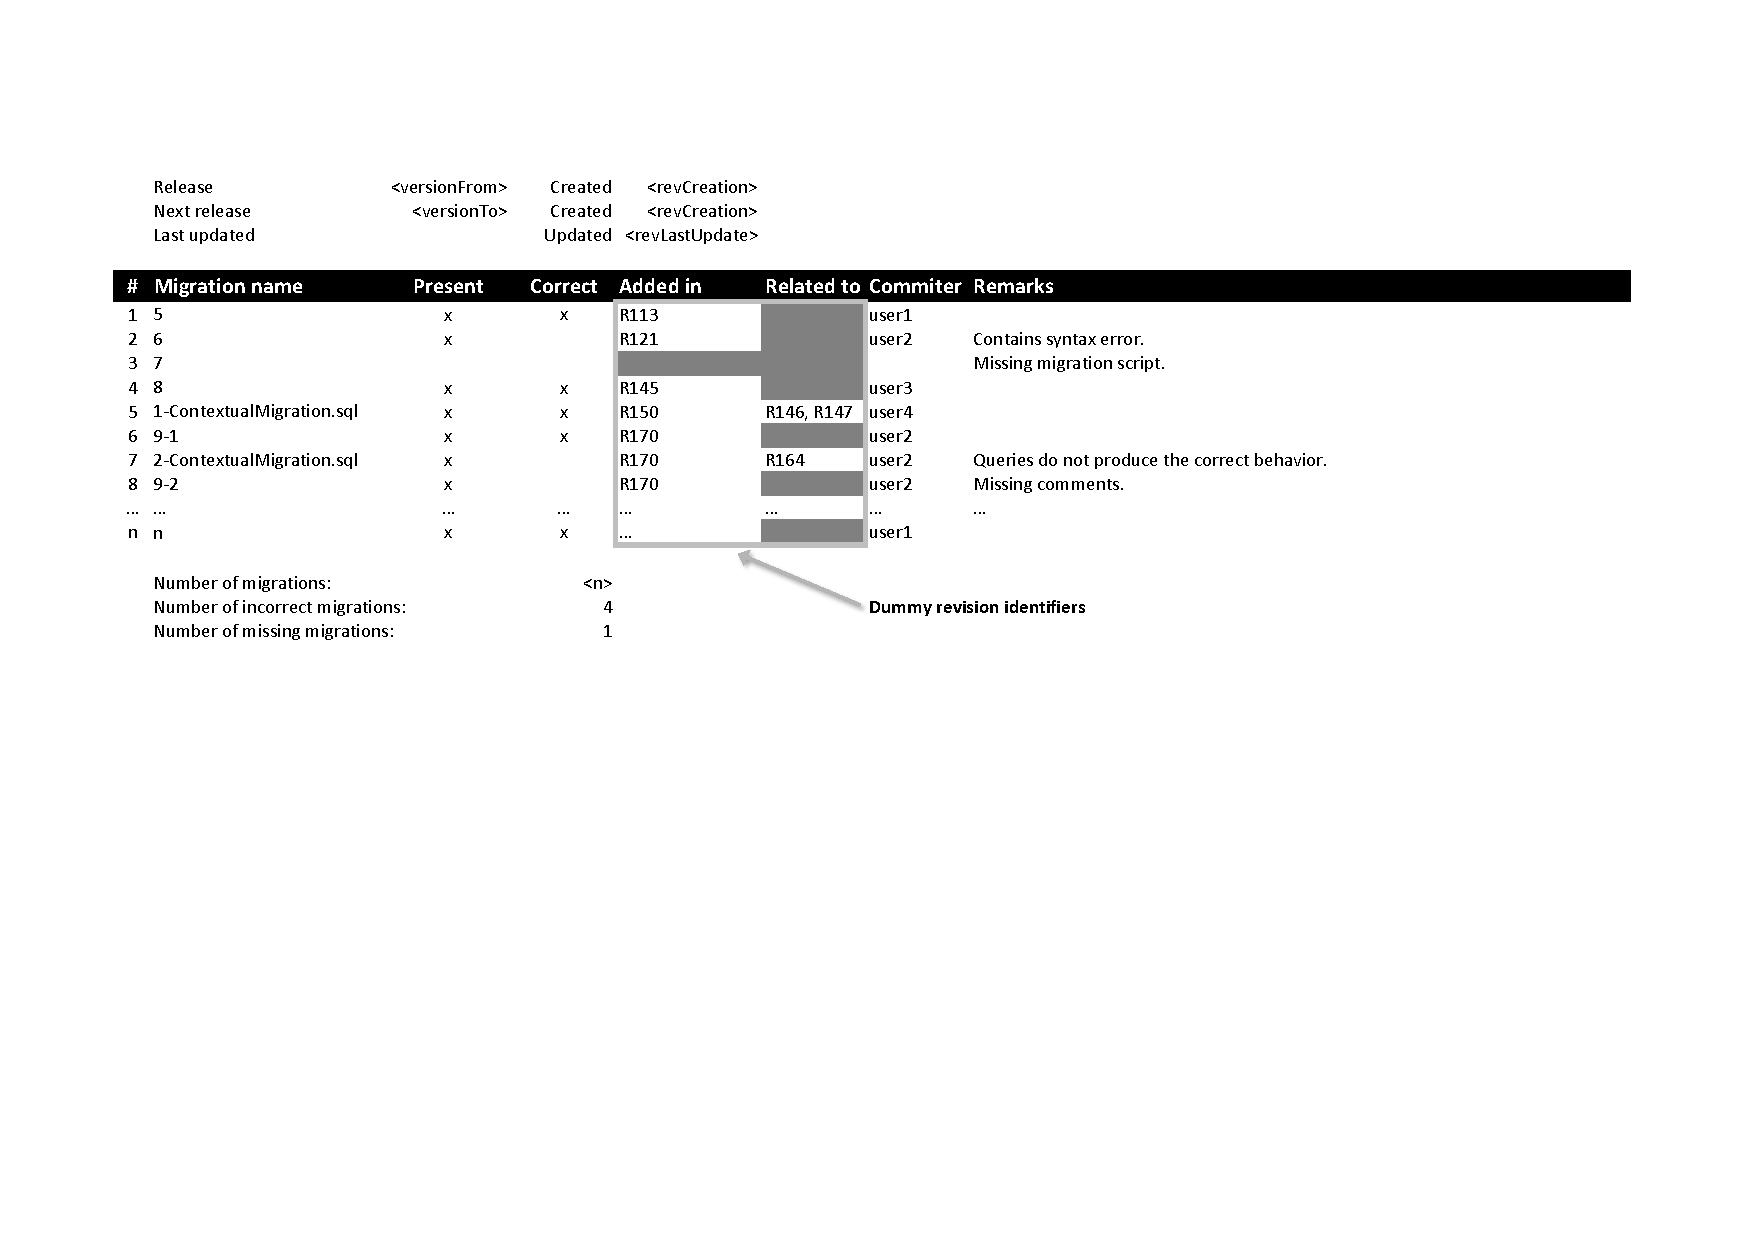
\includegraphics[scale=0.55]{images/MigrationMonitoringTemplate.pdf}
        \caption{Migration monitoring template}
        \label{fig:migTemplate}
\end{figure}

\subsubsection{Migration script writing rules\\}
	\label{sec:rules}

To write a migration script, we need to follow some rules for coherence, easiness and not the least important aspect, to match the format that the migration builder tool use to build the final migration script from the different migration script parts. We will go across the process that define how to write a script, how to name it and such of things. The figure \ref{fig:genMigScriptSchema} will show the whole process to write a script with references to other figures shown after. The figures \ref{fig:genMigScriptSchema-1}, \ref{fig:genMigScriptSchema-2}, \ref{fig:genMigScriptSchema-3} and \ref{fig:genMigScriptSchema-4} will show parts involved in figure \ref{fig:genMigScriptSchema}.

\begin{figure}[h]
        \centering
        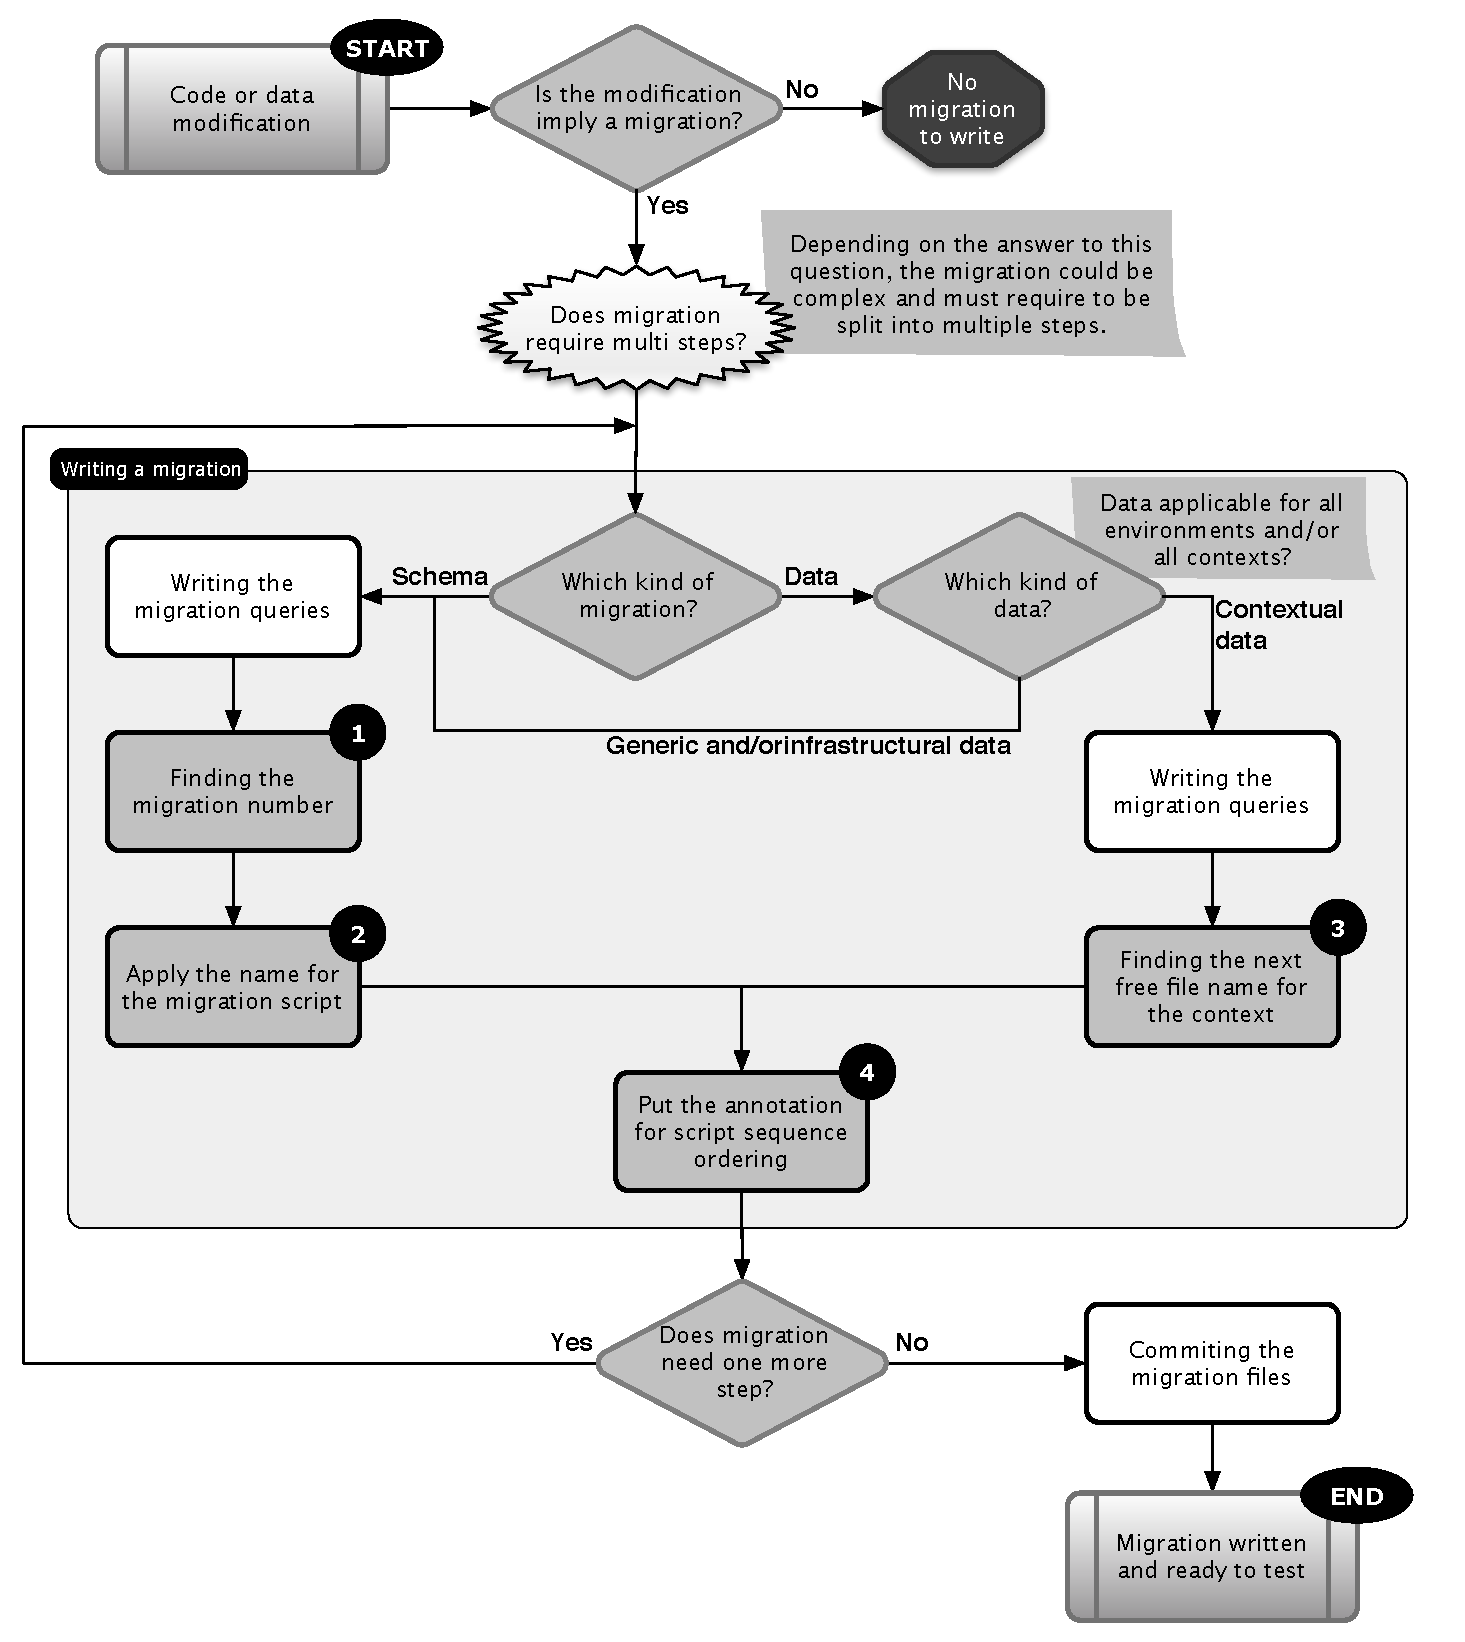
\includegraphics[scale=0.60]{images/mig-schema-gen-main.pdf}
        \caption{How to write a migration script schema}
        \label{fig:genMigScriptSchema}
\end{figure}

As we already discussed, we track the model modification through the help of some script and tools, but the developer who wrote the model modification has the responsibility to provide the corresponding migration script on his own (with the help of his colleagues if necessary). To help him in this task, some rules are in place to know where to put the queries and how to organize the migration. When a script is written, the developer must ask himself some questions to know how to organize his migration script. For example, the first question to ask is if a migration must be split or not?

Why a script could required more than one part? The reason is quite simple. When you manage multiple environments with the same application deployed with their own database (same schema across the different deployments), the data stored are not the same. They could be updated differently from environment to environment. Contextual requirements must be took into account. In this case, when the queries must manipulate the data in a contextual way, splitting migration script into parts is required. Sometimes, this question is not so easy to answer when the developer starts to write his queries. Our writing rules cover this case.

Before starting the script writing, the developer must answer one more question. Which kind of migration is it? Is it schema migration only? Is it migration and data? Is it data only? When there are data migration, the developer must also answer the question about the context of the data. Is the data generic/infrastructural or data are contextual to an environment? Based on the answers given by the developer, the process to write the migration script is slightly different.

Let's continue with an example to go deeper in the migration writing rules. Read the class diagrams on Fig. \ref{fig:classDiagSample} that shows before and after a code modification with impact on the database schema and data. In the "before" modification, we see a simple class that contains a price and a currency in "hardcoded" way. When the modification is done, the data model is better and contains relations between classes to enrich the way to store the data in a cleaner manner. The modification will also add an attribute type to categorize the products. This is probably not the best way to do this kind of modification but it is clearly much simpler for the demonstration for this paper.

\begin{figure}[h]
        \centering
        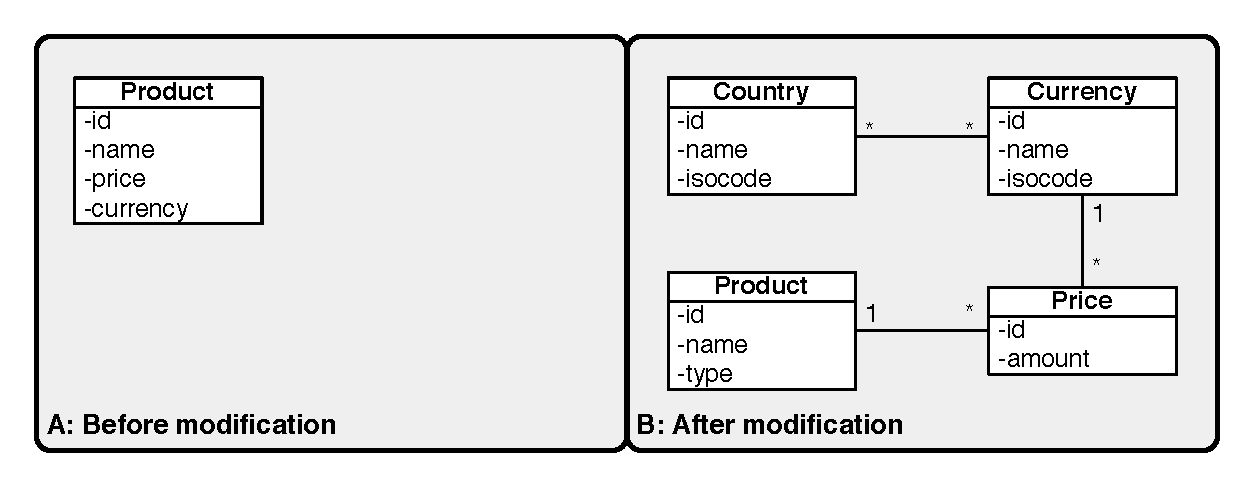
\includegraphics[scale=0.60]{images/ClassDiagramSample.pdf}
        \caption{Class Diagram Sample (before and after modification)}
        \label{fig:classDiagSample}
\end{figure}

With this example, we can clearly see that there are structural modifications but also data migration is required. There are some generic data and some contextual data. For example, the attribute type in the product class required to be updated depending on the data that are in the table at the time of the migration. This could be really tricky to update due to number of products already present in the table. Let assume that there is not a lot of data and that we could be able to write by hand the migration script. We can imagine that there is only ten products in the product table as the Fig. \ref{fig:classDiagDataBefore} shows the product table content before migration. The product tables contains vegetables and fruits (that will be stored later under type attribute). We did a simplification for the type attribute, we clearly imagine to create a class to store this data for cleaner approach of this data model. The script to create the table is shown on Listing \ref{list:classDiagSqlBefore}.

\begin{figure}[h]
        \centering
        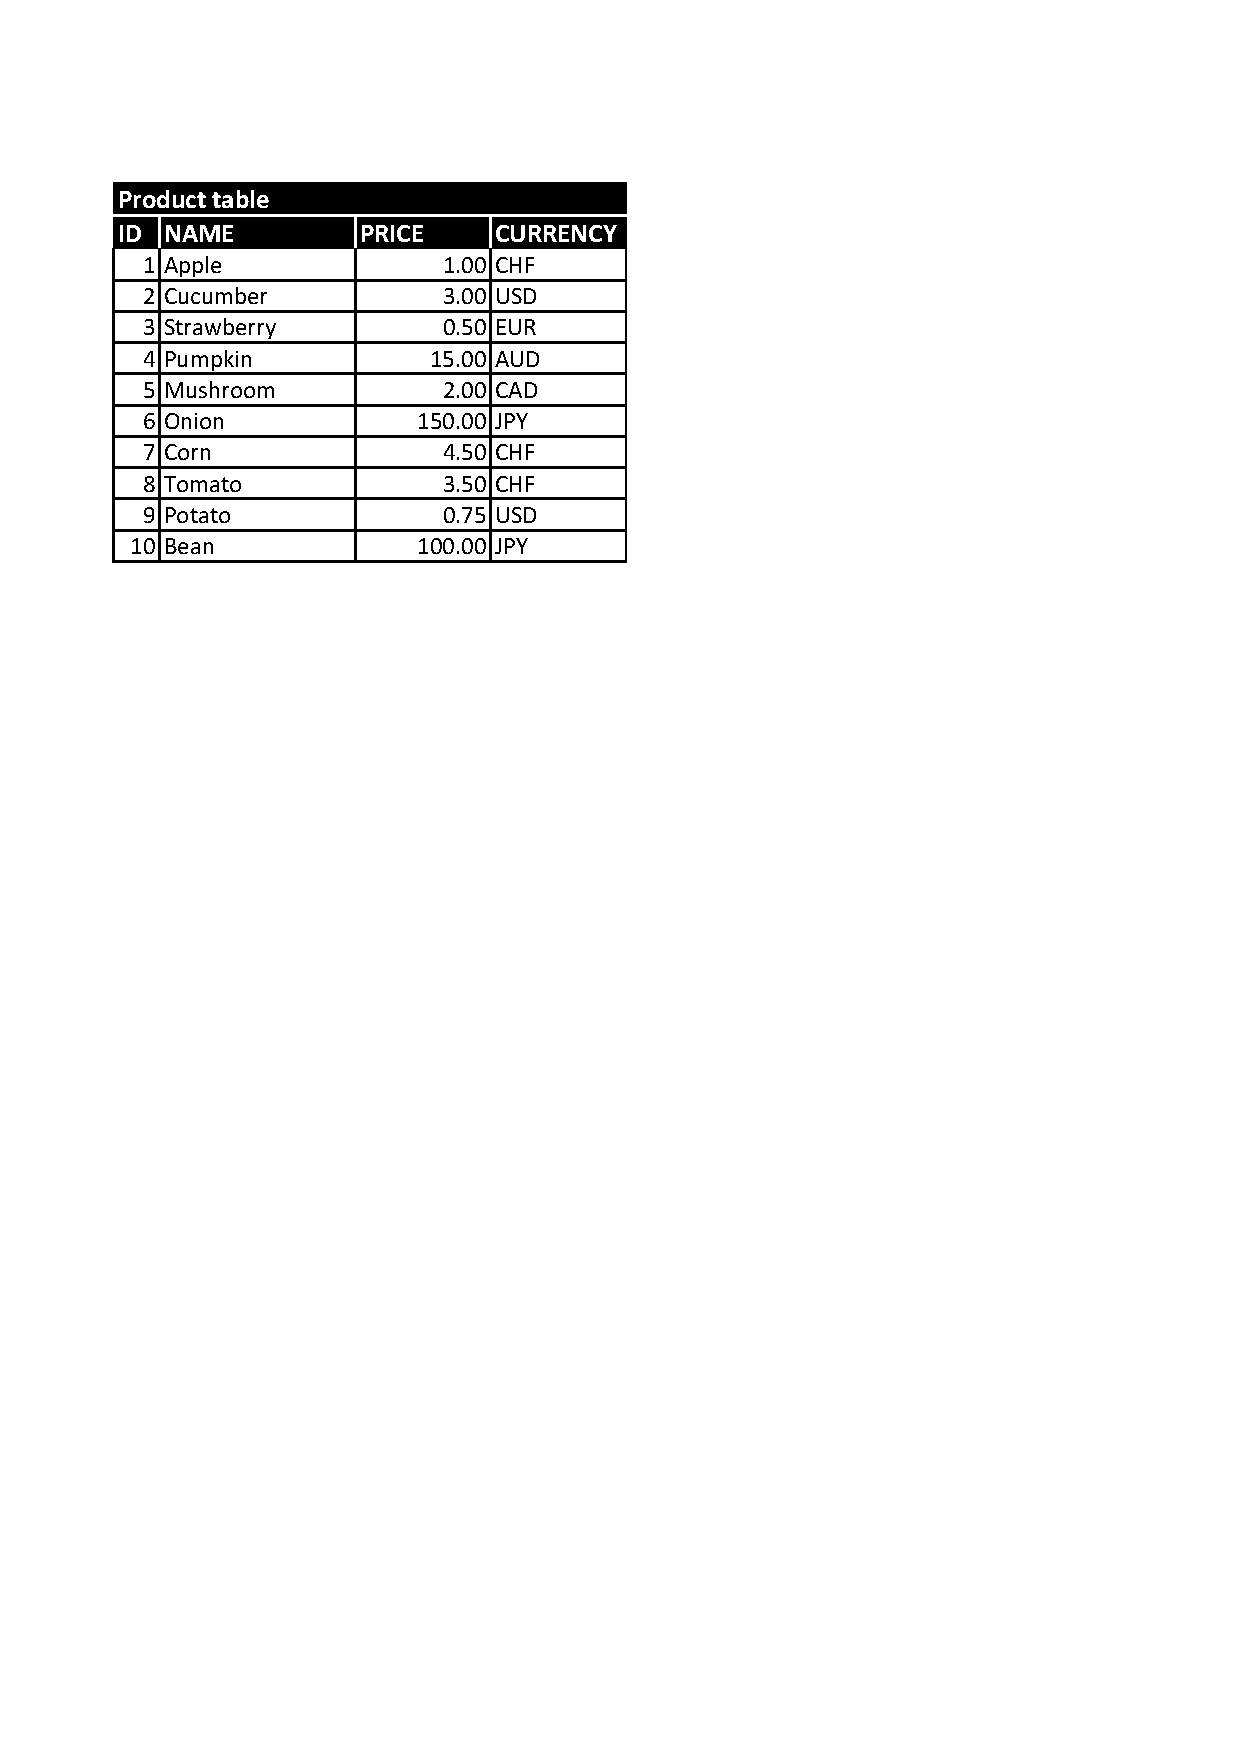
\includegraphics[scale=0.60]{images/ClassDiagramDataBefore.pdf}
        \caption{Class Diagram Sample - Data before modification}
        \label{fig:classDiagDataBefore}
\end{figure}

\lstinputlisting[label={list:classDiagSqlBefore}, caption={Class Diagram Sample - Schema before modification}, style={sqlStyle}]{sql/ClassDiagramSchemaBefore.sql}

Keep again an eye on the Fig. \ref{fig:genMigScriptSchema} and let's start with the migration writing. We know that the modification clearly implies a migration scripts. Does migration require multi steps? We are not sure at this step (or let assume that for the example). Which kind of migration is it? We have added classes and it implies schema update. So we are sure that there is a schema migration script. We also see that we need to add new data to fill the new tables implied by the migration. Is these data generic and/or infrastructural? Yes, they are for the Country and Currency tables. We also think about the price table that requires a major work to transform the data from Product table to Price table. At this cogitation, we discover that the type attribute must be filled depending on the data stored in the product table.

Finally, with this short example, we cover different the migration possibilities, schema, generic/infrastructural data and contextual data. At this stage, the developer must think about the migration ordering. It means that the queries must be ordered to be run correctly against the database that already contains data. Basically, we need to update the schema, adding new infrastructural data, migrate actual data and finally correcting/removing constraints/data. With our answers and reflexions, we clearly see that the script cannot be run in one part. We already know that we need to decompose our script into different parts. But first of all, let's go with the schema creation request. The queries could be seen on Listing \ref{list:classDiagMigrationStep1a}.

\lstinputlisting[label={list:classDiagMigrationStep1a}, caption={Class Diagram Sample - Schema migration - Step 1a}, style={sqlStyle}]{sql/ClassDiagramMigrationStep1a.sql}

At this step, we are ready to write the queries to populate the data that are generic/infrastructural. The countries and currencies are, in general, structural data that could be used in any environment. The queries (extract) could be viewed on Listing \ref{list:classDiagMigrationStep1b}. We also provide a query to extract the data for the three tables as we can view on Fig. \ref{fig:classDiagMigrationStep1bData}. We could discuss about the correctness of the hypothesis that the data are shared between different application deployment. We assume this is the case and that we use the same data in different deployments for this example.

\lstinputlisting[label={list:classDiagMigrationStep1b}, caption={Class Diagram Sample - Data migration - Step 1b}, style={sqlStyle}]{sql/ClassDiagramMigrationStep1b.sql}

\begin{figure}[h]
        \centering
        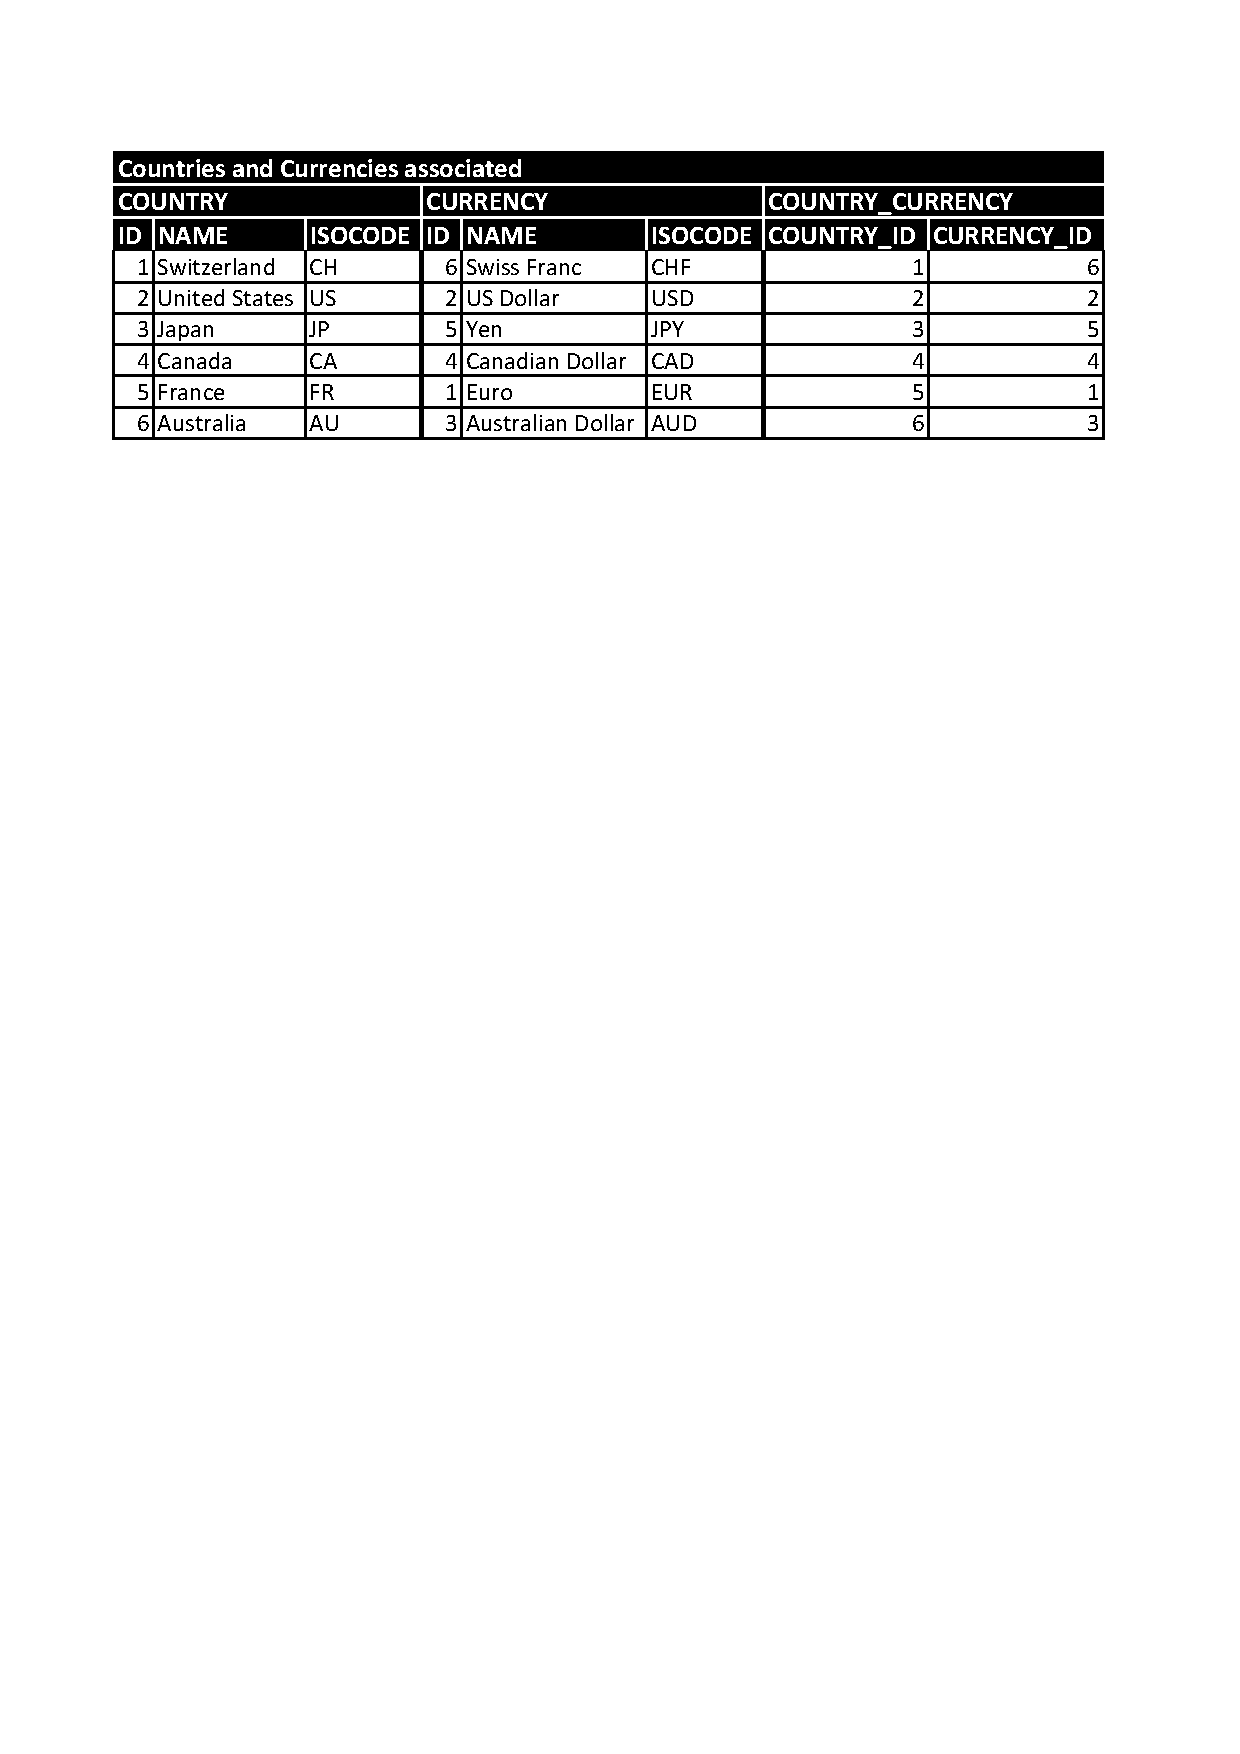
\includegraphics[scale=0.60]{images/ClassDiagramMigrationStep1bData.pdf}
        \caption{Class Diagram Sample - Resulting data - Step 1b}
        \label{fig:classDiagMigrationStep1bData}
\end{figure}

We have also to insert the prices in the Price table before removing the columns. The queries could be viewed on Listing \ref{list:classDiagMigrationStep1c}. The queries could be done independently from the context. In any application deployment that has products, they are prices and currencies to convert/migrate. This job could be done by queries that are not dependents to the application deployment.

\lstinputlisting[label={list:classDiagMigrationStep1c}, caption={Class Diagram Sample - Schema and migration data - Step 1c}, style={sqlStyle}]{sql/ClassDiagramMigrationStep1c.sql}

So we have written the queries involved in the first step of the migration that add the new tables, add the constraints and add the data column to the existing entity. We also added the infrastructural data. Now, we have to place these queries to the right place. The Fig. \ref{fig:genMigScriptSchema-1} will help us to retrieve the migration number that we will use to situate the script into our migration process. We have simply to know where the modification is done. In our case, we suppose that the modification are done in working trunk directory of our versioned repository. Otherwise, we should get the migration number from the Branch/Release path and apply the rules for this situation. For the following paragraphs, we assume that the next migration number is 15.

\begin{figure}[h]
        \centering
        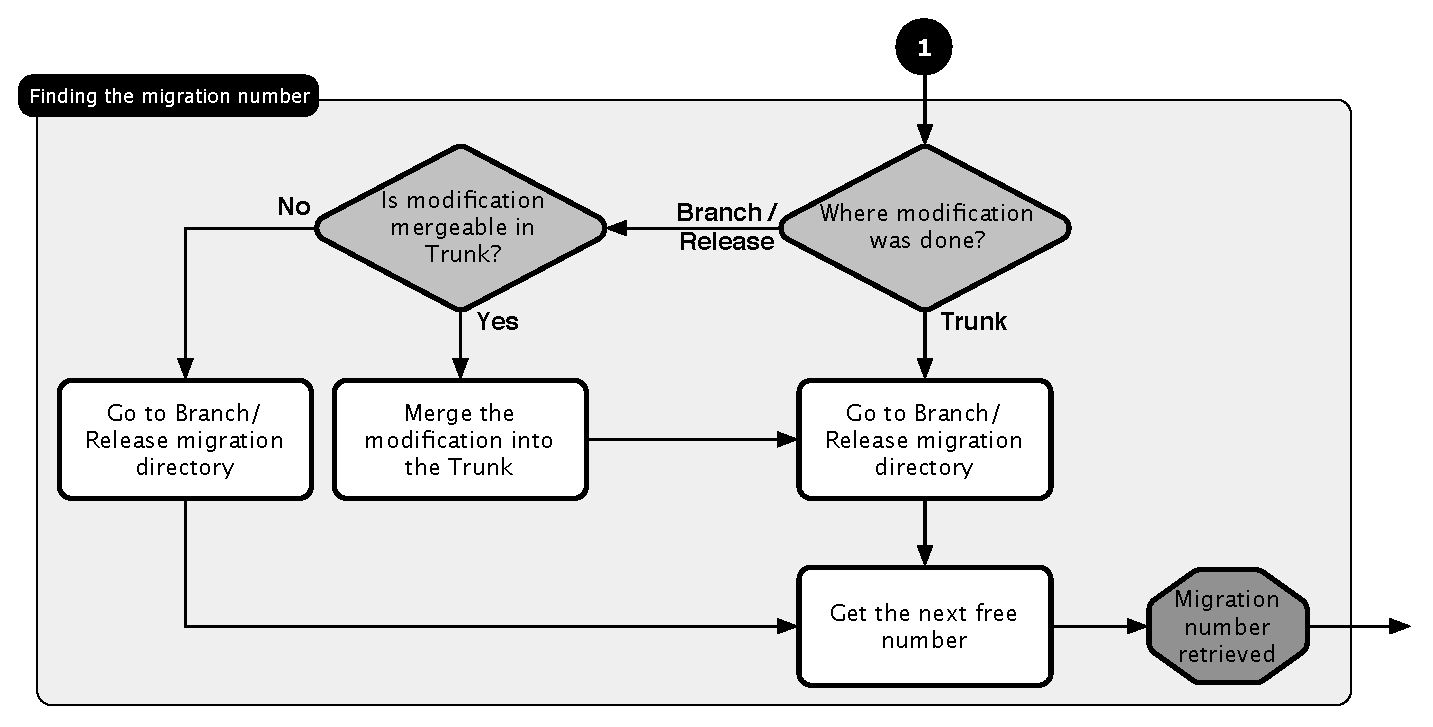
\includegraphics[scale=0.60]{images/mig-schema-gen-1.pdf}
        \caption{How to write a migration script schema - Subpart 1}
        \label{fig:genMigScriptSchema-1}
\end{figure}

When the migration number is retrieved, we can create the file to store the queries for the migration step. So, now, we need to follow the rules to build the migration name that could be viewed on Fig. \ref{fig:genMigScriptSchema-2}. Is there already a script for the migration (migration number we just previously retrieved)? In our case, we have only one script yet, so we need to build the name as "15.sql". A shortcut could be taken to build the script name because we already know that we will have another script for the same revision but for the example, we will strictly follow the rules.

\begin{figure}[h]
        \centering
        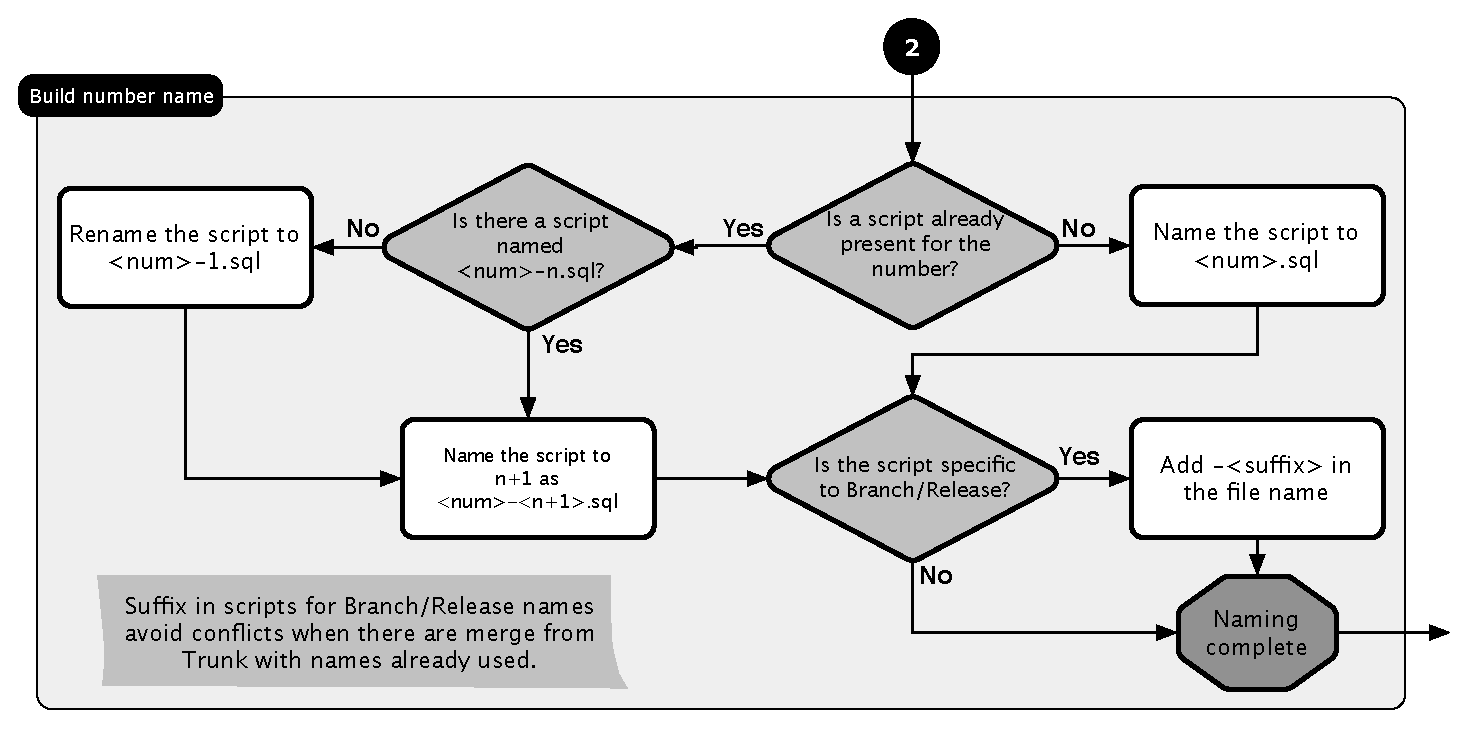
\includegraphics[scale=0.60]{images/mig-schema-gen-2.pdf}
        \caption{How to write a migration script schema - Subpart 2}
        \label{fig:genMigScriptSchema-2}
\end{figure}

In some situations, we need to add an information to influence the migration scripts ordering. Imagine that you did a correction into a release version in revision identifier 245 and you merged the correction in your trunk in revision identifier 253, you will have a migration script name like n.sql (or eventually n-<suffix>.sql if the correction was not planed to be merged into the Trunk). Some other scripts could be already present in the Trunk migration directory that you do not want they could be run before the script you just merged. For this reason, we introduce some annotations to help the script parts ordering. This mechanism is more largely used in the contextual scripts due to the naming conventions we used that is different from the migration number system. With @after and @before annotations placed in the comments of the migration part script, we are able to define precisely where a migration script must be run when the place is different from the normal one. The Fig. \ref{fig:genMigScriptSchema-4} shows how to use the annotations we have introduced. This system is designed to be used by some tools to help the concatenation of the different script parts. For the current migration script step, we do not need to specify any annotations for a special ordering.

\begin{figure}[h]
        \centering
        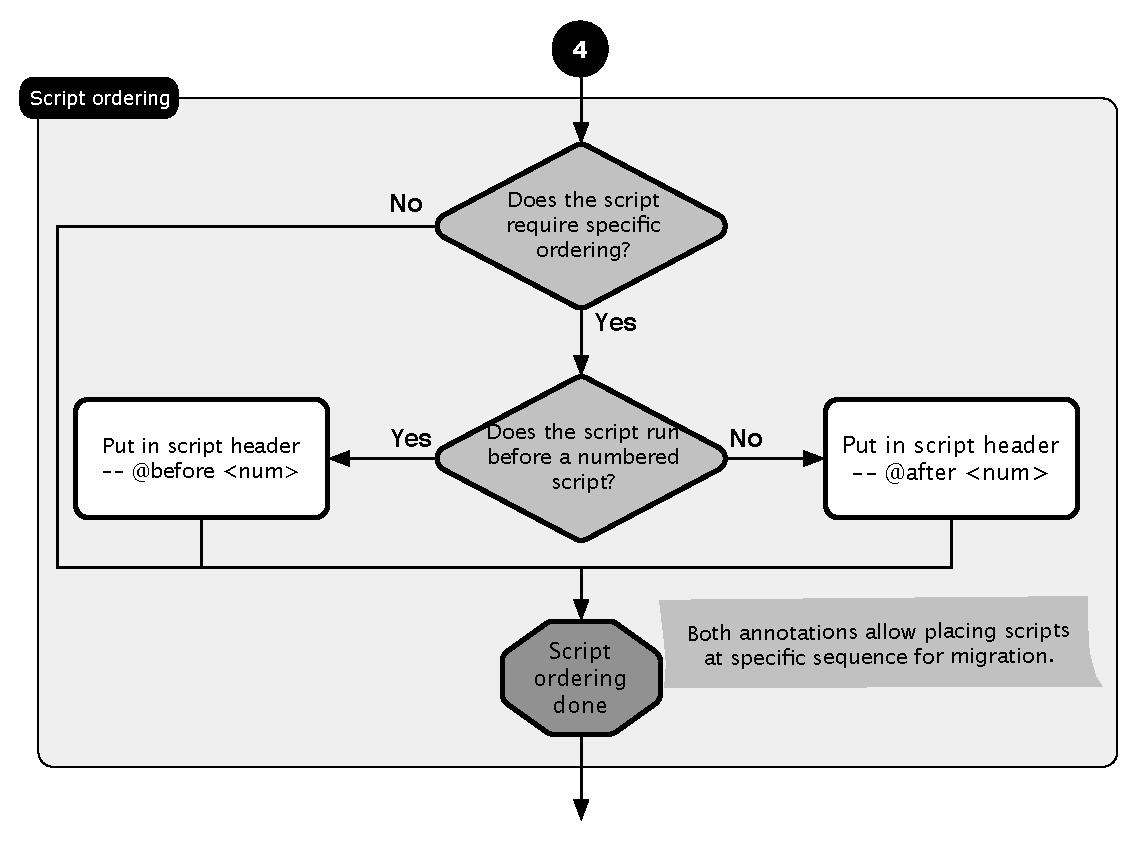
\includegraphics[scale=0.60]{images/mig-schema-gen-4.pdf}
        \caption{How to write a migration script schema - Subpart 4}
        \label{fig:genMigScriptSchema-4}
\end{figure}

We have finished one loop of the process to write a migration script entirely. We need to iterate, at least, one more time for the contextual data (data present in product table). So the Fig. \ref{fig:genMigScriptSchema} give us the next step to follow. This time we need to write contextual queries. The queries are not so complicated but depends entirely on the data present in the table product. We need to write the queries to add the type to each product. The Fig. \ref{list:classDiagMigrationStep2} shows an extract of the queries we have to write. For the example, the queries shown are specially simple and quite stupid, we can construct a better script that will be able to define the type of products based on the name with a lookup table for example but this kind of considerations is out of the scope.

\lstinputlisting[label={list:classDiagMigrationStep2}, caption={Class Diagram Sample - Migration data - Step 2}, style={sqlStyle}]{sql/ClassDiagramMigrationStep2.sql}

Now that we have the queries, one more time, we need to place the migration script at the right place. For that, we will follow the rules on Fig. \ref{fig:genMigScriptSchema-3}. We have to go to the right directory. First of all, we have, on the versioning repository, a dedicated directory to store the contextual migration scripts. We go into this directory. Then, we have to check if the directory for the environment we want to update is created, if not, we create the directory. By default, we use a dummy environment called "local" or "dev" to store the scripts before they will be adapted to the right environment. When the scripts are written, it is unusual that we already know for which environment we have to write the migration script and even if we know, until we have to migrate the environment, the data could change and the script could be not relevant. So, we will always create the contextual migration script into this dummy environment to be up to date with the migration monitoring. Generally, in multiple environment, the application deployment is not easy to follow because each environment could evolves differently. Each one could have a different version that requires a specific migration script based on the different migration script parts.

In the environment directory, we will check if a directory exists for the version deployed currently on the environment (called version from). If the directory does not exist, we will create it. And finally, we could check if a migration script already exist or not. If no, we will have a script name like "1-$<$FreeText$>$.sql" otherwise we will have "$<$LastNumber$>$+1-$<$FreeText$>$.sql".

In our example, we assume that we wrote the first contextual script for the dummy environment and version from which the next migration will be done. So, our script name will be like "1-AddTypeToProducts.sql". After that, we have just to go through the ordering rules to add an annotation to put the script just after the step one we just wrote before this one. We will add "-- @after 15-1" (Remember that the "-1" will come later due to the fact that the migration is split in two parts due to null constraint not addable when there are data with no default value).

\begin{figure}[h]
        \centering
        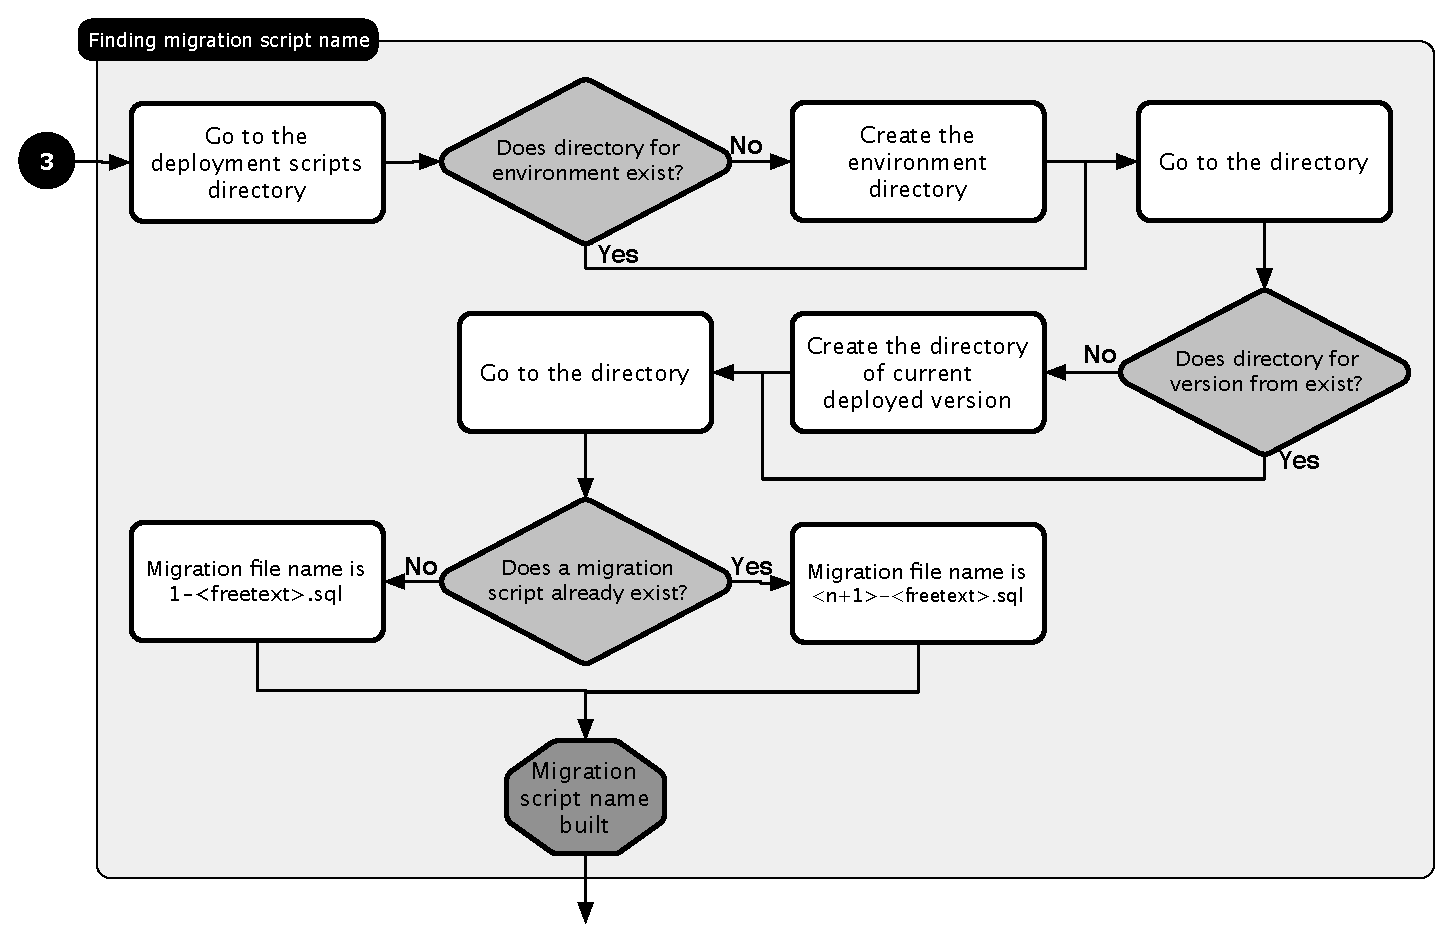
\includegraphics[scale=0.60]{images/mig-schema-gen-3.pdf}
        \caption{How to write a migration script schema - Subpart 3}
        \label{fig:genMigScriptSchema-3}
\end{figure}

Finally, we can conclude the migration with a final query to add the missing constraint on the column type on Product table shown on Listing. \ref{list:classDiagMigrationStep3} that we was not able to do before updating the Product data. So we will go through the rules diagrams again. When we have to find the name of the migration script step (based on the Fig. \ref{fig:genMigScriptSchema-2}) we see that there is already a script named "15.sql". So we need to rename the script to "15-1.sql" (as we already anticipated in the previous paragraph). When it is done, we will find the name for this step as "15-2.sql". That is all. We have finished to prepare the migration scripts. To finalize the migration writing process, we have just to commit the files into the versioned repository.

\lstinputlisting[label={list:classDiagMigrationStep3}, caption={Class Diagram Sample - Schema migration - Step 3}, style={sqlStyle}]{sql/ClassDiagramMigrationStep3.sql}

From now, we have a lot of migration scripts distributed across different files. When we will run a migration, we need to concatenate the files we want in the order required. This part is really tricky if it is done by hand. In the \autoref{sec:buildingScript} we provide a solution that could be used to automatize the concatenation of the migration scripts. The ability to have the different files allows building at any time, for any version, at any level a new application deployment. It becomes easy to deploy a new application in a new environment with the scripts that are able to prepare the database for the application.

\subsection{Tools}

To support the different processes defined previously, we need tools to help us. We provide some conceptual tool ideas that we could use.

\subsubsection{Code modification detection\\}

As we explained, we need the ability to detect code modification but especially modifications that have impact on the database schema and/or data. Generally, application code is such well organized that these modifications are easy to monitor with some addition to the versioning system in place. It is relatively easy to write plugins or scripts that add this logic to the versioning system with the ability to send emails with the potential matches triggered.

The persons in charge of code monitoring must have the information to quickly decide if a modification has an impact or not on the migration process. For that, the emails sent must contain at least the list of files impacted by code modifications. If the differences between two modifications is provided, the work to analyze what is implied in a migration is really more easy. The pseudo code \ref{pcode:monitoringPseudo} show a basic mechanism to monitor the code changes by a succession of filtering to include the path that have some interest and to exclude some of them in the result of inclusive filters. This allow getting only the files that are useful. The remaining code is present to prepare the result with the relevant information to help differentiate the database impacts.

\begin{algorithm}
	\caption{Code monitoring}
	\label{pcode:monitoringPseudo}
	\begin{algorithmic}[1]
		\State \tdefine{inclusiveFilter}{Path to include}
		\State \tdefine{exclusiveFilter}{Path to exclude}
		\State
		\State \Comment{Retrieve information from versioning system for the current version}
		\State \tdefine{changedFiles}{\Call{retrieveChangedFiles}{~}}
		\State
		\State \Comment{Apply filters to keep only relevant files}
		\State \tdefine{tempFiles}{\Call{applyInclusiveFilter}{\tvar{changedFiles}, \tvar{inclusiveFilter}}}
		\State \tdefine{remainingFiles}{\Call{applyExclusiveFilter}{\tvar{tempFiles}, \tvar{exclusiveFilter}}}
		\State
		\State \Comment{Prepare an email to send the code monitoring result}
		\State \Call{createEmail}{~}
		\State
		\State \Comment{Check if there are relevant files}
		\If{\tvar{remainingFiles} not empty} 
			\State \Call{addToEmail}{\tvar{remainingFiles}}
			\State
			\State \Comment{For all relevant files, extract the difference from previous modification}
			\ForAll{\tvar{changedFile} in \tvar{remainingChangedFiles}}
				\State \tdefine{result}{\Call{retrieveDifferenceFromPrevious}{\tvar{changedFile}}}
				\State \Call{addToEmail}{\tvar{result}}
			\EndFor 
		\EndIf
		\State
		\State \Call{sendEmail}{~}
	\end{algorithmic}
\end{algorithm}

As we seen, this conceptual tool is really simple to develop and put in place for basic requirements. It is also easy to improve and add additional monitoring. The only pre-requisite is to have a versioning system that allows to add plugins or hooks. If it is not the case, it is required to add mechanism to do this monitoring. For example, a scheduled monitoring everyday could be a solution if there is no way to integrate this tool in the versioning process.

\subsubsection{Migration info and statitics\\}
	\label{sec:migInfoAndStats}

When a migration is ready to be used, another requirements is to track the queries executed to allows gathering statistics as the duration of queries, the number of queries and such of things. In testing environment, it could allow to retrieve where a script loose to much time and which queries are costly. In addition, we can also store some data as the version from which we migrate and the version to which we migrate. We can store the versioning range identifiers for the migration.

For a relevant usage of these data, we need to store them directly in the application database in each environments. It offers a way to get information in real time at any time for any environments. In addition, if the application contains an admin interface, it could be integrated to it.

We have modeled the solution as shown in Fig. \ref{fig:migInfo}. Our solution is sufficiently generic that could be adapted to any use with small changes. We have one table that store the migration info (version from, version to, versioning start identifier, versioning end identifier, number of queries, duration, date start, date end). A second table that stores the metrics retrieved during the migration execution like number of inserts, updates and so on. The third table stores the different parts of a migration script with their duration. This table stores the details of migration execution that allows to know which script could be a bottleneck.

\begin{figure}[h]
        \centering
        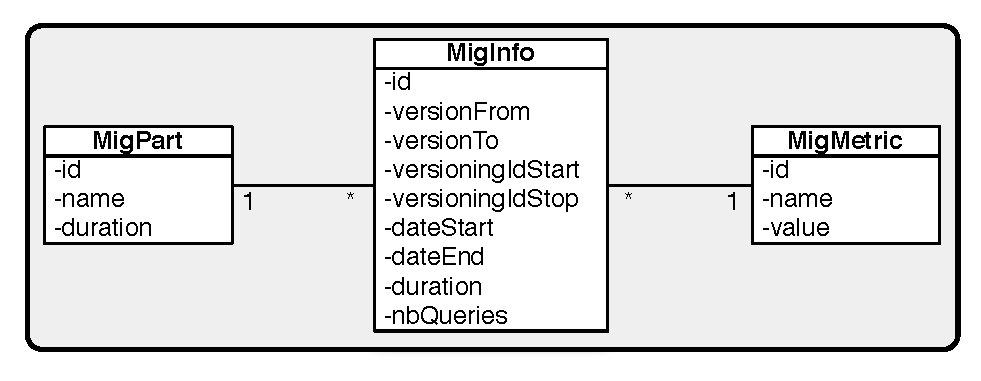
\includegraphics[scale=0.80]{images/MigrationInfo.pdf}
        \caption{Migration Info Model}
        \label{fig:migInfo}
\end{figure}

\subsubsection{Building tool\\}
	\label{sec:buildingScript}

To help the process to deploy a new application, we provide some algorithms to help to prepare the final script built from various migration parts. As we already discussed in \autoref{sec:rules}, we have added some logic to help the scripts ordering with annotations. These annotations could be placed in any script part. To build the final script, we need some information to retrieve the scripts and to do the correct sorting of scripts. We need to know the version from which we are migrating and also the version where we will be after the migration. The migration script number start and end are required to scope the migration script parts we will use. The environment is required to get the contextual script for the migration. Last but not the least, we need to know the application to migrate (and its database name). We need also to know if it is required to get the initial database creation with initial data population. What does it mean?

Up to now, we have discussed about migration but we need also to cover the first application deployment that is really similar with a major difference. In the development cycle, we do not want to manage migration scripts until it becomes required. We want to write migration scripts only when they are needed. For this reason, until the first deployment, we only write code without corresponding migration scripts. At the first deployment, we will create two files in the same way of normal migration scripts called "\_db\_creation.sql" and "\_db\_data\_init.sql". The first file contains the database schema corresponding to the application state at the deployment time. The second file contains the data corresponding to the schema and deployment needs. Eventually, some of data from this file must be placed in a contextual file as we already discussed.

With this approach, we keep agility to write code quickly until we have to deploy the application in a production environment. We could refactor any part of the application as we want without worrying about the consequences on migrations. At the first deployment, the application becomes "migration managed" application and needs to enter in the whole process we described. The both files are added at the final script beginning only if the building tool is asked for. We need to tell the tool if the application must be initialized or not.

Based on the different information gathered, we could build the runnable migration script. During the building process, we add some information as we have just discussed in the previous \autoref{sec:migInfoAndStats}. This data populates the different tables related to the migration information and statistics. The queries added are part of the runnable migration script. The pseudo codes \ref{pcode:buildingScript1}, \ref{pcode:buildingScript2}, \ref{pcode:buildingScript3}, \ref{pcode:buildingScript4} and \ref{pcode:buildingScript5} show how the building tool works.

In the pseudo code \ref{pcode:buildingScript1} we show how are the inputs required by the script tool to build the final migration script. We also get the migration part files directly from the versioning system to be sure to have the latest script parts. We initialize an empty list to store the resulting list of migrations to be include in the current migration. One part of the script, allows adding the initial database schema creation with initial data (like infrastructural and configuration data). This part is optional and could be configured when the script is called. 

\begin{algorithm}
	\caption{Builiding tool - Part 1 - Definitions}
	\label{pcode:buildingScript1}
	\begin{algorithmic}[1]
		\State \Comment{User inputs}
		\State \tdefine{versionFrom}{Get the version from}
		\State \tdefine{versionTo}{Get the version to}
		\State \tdefine{startNum}{Get the start number}
		\State \tdefine{endNum}{Get the end number}
		\State \tdefine{envir}{Get the environment}
		\State \tdefine{appName}{Get the application name}
		\State \tdefine{appDbName}{Get the application database name}
		\State \tdefine{initialize}{Get the application initialized or not}
		\State
		\State \Comment{Interaction with the versioning system}
		\State \tdefine{migrationFiles}{\Call{retrieveFromVersioningSystem}{\tquote{migration files}}}
		\State \tdefine{contextualFiles}{\Call{retriveFromVersioningSystem}{\tquote{contextual migration files}}}
		\State
		\State \Comment{List to store the migration parts in a ordered way}
		\State \tdefine{orderedList}{\O}
		\State
		\State \Comment{Add initial scripts if required}
		\If{\tvar{initialize}}
			\State \Call{addAtEnd}{\tvar{orderedList}, \tquote{\_db\_creation.sql}}
			\State \Call{addAtEnd}{\tvar{orderedList}, \tquote{\_db\_data\_init.sql}}
		\EndIf
		\algstore{bkbreak}
	\end{algorithmic}
\end{algorithm}

The second part of the building tool shown on pseudo code \ref{pcode:buildingScript2} manage the migration script parts that could be applied on every deployments. We assumes that the list of files analyzed is already sorted in the chronological order of numbering info. For each file, we check that is or not in the scope of the configured migration. We keep only the ones that are in the scope. For the others, we check the annotations in the files to see if they could be integrated to the current migration or not.

\begin{algorithm}[h]
	\caption{Builiding tool - Part 2 - Migration files}
	\label{pcode:buildingScript2}
	\begin{algorithmic}
		\algrestore{bkbreak}
		\State \Comment{Analyze migration files}
		\ForAll{\tvar{migrationFile} in \tvar{migrationFiles}}
			\State \tdefine{migrationNumber}{\Call{getMigrationNumber}{\tvar{migrationFile}}}
			\State
			\State \Comment{File is in the range of scripts wanted}
			\If{\tvar{migrationNumber} $\geq$ \tvar{startNum} \&\& \tvar{migrationNumber} $\leq$ \tvar{endNum}}
				\State \Call{addAtEnd}{\tvar{orderedList}, \tvar{migrationFile}}
			\ElsIf{\Call{containsAnnotation}{\tvar{migrationFile}}}
				\State \Comment{See pseudo code \ref{pcode:buildingScript4}}
				\State \Call{analyzeFile}{\tvar{orderedList}, \tvar{migrationFile}, \texttt{False}}
			\EndIf		
		\EndFor
		\algstore{bkbreak}
	\end{algorithmic}
\end{algorithm}

In the third part shown on pseudo code \ref{pcode:buildingScript3}, we analyze the contextual migration parts. The mechanism is pretty the same as the previous analysis. The difference remains in the analyze file procedure that trigger if the file is contextual or not. We will discuss about that a little later.

\begin{algorithm}[h]
	\caption{Builiding tool - Part 3 - Contextual files}
	\label{pcode:buildingScript3}
	\begin{algorithmic}
		\algrestore{bkbreak}
		\State \Comment{Analyze contextual files}
		\ForAll{\tvar{contextualFile} in \tvar{contextualFiles}}
			\State \Comment{See pseudo code \ref{pcode:buildingScript4}}
			\State \Call{analyzeFile}{\tvar{orderedList}, \tvar{file}, \texttt{True}}
		\EndFor
		\algstore{bkbreak}
	\end{algorithmic}
\end{algorithm}

Finally, when the ordered list of migrations files is ready, we could build the final script with some additions for the migration process. In the pseudo code \ref{pcode:buildingScript4} we show how the final script is built. We prepare a file with a header that contains a part that we call manifest. This manifest contains all relevant data used to build the final script and to have tracking data. For example, we will store the version from and to, versioning identifiers, creation date and the list of migration script parts we have in the final migration file. We also prepare some statements for statistical purposes. After that, for each file we add in the final one, we add some comments to create sections in the file to be userfriendly readable. Each migration part is separate by a header and footer that scope the migration part in the final file. The listing \ref{list:resultingFile} shows a result that could be produced by the building tool. We also add some metric queries for the current migration script (for example, we triggered the time duration of the current migration script part into the whole migration script. And finally, we add a final footer that contains the queries to populate the different migration tables in the application database.

\begin{algorithm}[h]
	\caption{Builiding tool - Part 4 - Build final script}
	\label{pcode:buildingScript4}
	\begin{algorithmic}
		\algrestore{bkbreak}
		\State \tdefine{finalScript}{\Call{createFinalFile}{~}}
		\State
		\State \Comment{Populate final file with statistical queries}
		\State \Call{addFileHeader}{\tvar{finalScript}}
		\State
		\State \Comment{Iterate in the chronological order}
		\ForAll{\tvar{file} in \tvar{orderedFile}}
			\State \Call{addHeader}{\tvar{finalScript}, \tvar{file}}
			\State \Call{addPreMigrationPartMetricQueries}{\tvar{finalScript}, \tvar{file}}
			\State \Call{addScript}{\tvar{finalScript}, \tvar{file}}
			\State \Call{addPosMigrationPartMetricQueries}{\tvar{finalScript}, \tvar{file}}
			\State \Call{addFooter}{\tvar{finalScript}, \tvar{file}}
		\EndFor
		\State
		\State \Call{addFileFooter}{\tvar{finalScript}}
		\algstore{bkbreak}
	\end{algorithmic}
\end{algorithm}

\lstinputlisting[label={list:resultingFile}, caption={Final migration script example}, style={sqlStyle}]{sql/migrationResult.sql}

The procedure to analyze the files to know if we need to keep them or not. For simplifications, we do not manage correctly the problem of transitivity. We mean that we do not follow the annotations across the script parts. If a script is annotated to be before one another script that also contains an annotation defining to be before one more script, we will lost the first annotated script with the pseudo code \ref{pcode:buildingScript5}. Some other case of transitivity are covered. It is relatively easy to modify our pseudo code handle this use case but the pseudo will become more complex to read. So, we retrieve the annotation number and the annotation type (after or before). If the annotation is in the range we have specified for the migration or the annotation is already in the range, we will add the file to the list. We have also to check if the list already contains a file for the annotation number, if this the case, we simply add the file after the one found otherwise we just add the file at the correct place relative to the annotation number. For the contextual scripts, we also check that if there is no annotation, we simply add them to the end of the list in the goal to manage them manually. The building tool could provide some mechanism to move manually some scripts before building the final script.

\begin{algorithm}[h]
	\caption{Builiding tool - Part 5 - Procedure to analyze annotated script parts}
	\label{pcode:buildingScript5}
	\begin{algorithmic}[1]
		\algrestore{bkbreak}
		\Procedure{analyzeFile}{\tvar{orderedList}, \tvar{file}, \tvar{contextual}}
			\State \tdefine{anNumber}{\Call{getMigrationNumberFromAnnotation}{\tvar{file}}}
			\State \tdefine{anType}{\Call{getAnnotationType}{\tvar{file}}}
			\State
			\State \Comment{Check if the annotation implies to add the file}		
			\If{(\tvar{anNumber} $\geq$ \tvar{startNum} \&\& \tvar{anNumber} $\leq$ \tvar{endNum}) \textbar\textbar~\tvar{anNumber} in \tvar{orderedList}} 
				\State \tdefine{fileFound}{\Call{findFileByNumber}{\tvar{orderedList}, \tvar{anNumber}}}
				\State
				\State \Comment{Check the file exists in the list}
				\If{\Call{isNotNull}{\tvar{fileFound}}}
					\If{\tvar{anType} = \tquote{@after}}
						\State \Call{insertAfter}{\tvar{orderList}, \tvar{fileFound}, \tvar{file}}
					\Else
						\State \Call{insertBefore}{\tvar{orderList}, \tvar{fileFound}, \tvar{file}}
					\EndIf
				\EndIf
			\ElsIf{contextual}
				\State \Comment{Add the script for manual processing}
				\State \Call{addAtEnd}{\tvar{orderedList}, \tvar{file}}
			\EndIf
		\EndProcedure
	\end{algorithmic}
\end{algorithm}
